\section{Reading the pushbutton Status from Scilab}
\subsection{Reading the pushbutton Status}
In this section, we discuss how to carry out the experiments of the
previous section from Scilab. We will list the same two experiments,
in the same order.  The shield has to be attached to the \arduino\ board
before doing these experiments and the \arduino\ needs to be connected to the computer 
with a USB cable, as shown in \figref{arduino}.
The reader should go through the instructions given in
\secref{sec:sci-start} before getting started. 
\begin{enumerate}
\item In the first experiment, we will read the pushbutton status using a 
Graphical user interface (GUI) in Scilab. The code for this experiment is 
given in  \sciref{sci:push-100}. As explained earlier in \secref{sec:light-sci}, 
we begin with serial port initialization. Then, we read the input coming from
digital pin 12 using the following command: 
  \lstinputlisting[firstline=4,lastline=4]
  {\LocPushscicode/push-button-status.sce} Note that the one leg of the pushbutton on
  the shield is connected to digital pin 12 of \arduino\, 
  as given in \figref{fig:pushbuttonconn}. The read value is displayed as a GUI using
  the following command: \lstinputlisting[firstline=5,lastline=5]
  {\LocPushscicode/push-button-status.sce} where {\tt val} contains
  the pushbutton value acquired by the previous command.
  When the pushbutton is not pressed, {\tt val} will be ``0''. On the other hand,
  when the pushbutton is pressed, {\tt val} will be ``1''. To
  encourage the user to have a good hands-on, we run these commands in
  a {\tt for} loop for 1000 iterations. While running this experiment, 
  the readers must press and release the pushbutton and observe the values being printed on the
  GUI, as shown in \figref{fig:ard-meter}.
 \begin{figure}
    \centering
    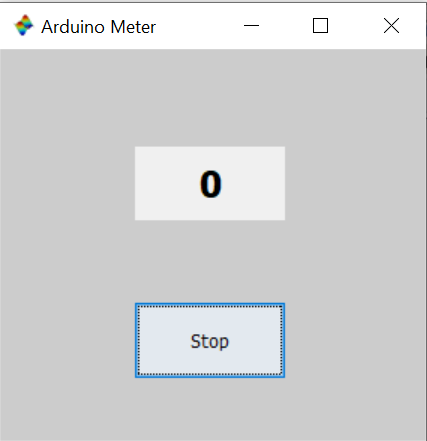
\includegraphics[width=\smfig]{\LocPushfig/sci-ard-meter.png}
    \caption{GUI in Scilab to show the status of the pushbutton}
    %\redcolor{connected on pin no. D12}}
    \label{fig:ard-meter}
  \end{figure}
\item This experiment is an extension of the previous
  experiment. Here, we control the state of an LED as per the status
  of the pushbutton. In other words, digital output to an LED is
  decided by the digital input received from the pushbutton. The code
  for this experiment is given in \sciref{sci:push-200}. After reading
  the pushbutton status, we turn the LED on if the pushbutton is
  pressed, otherwise we turn it off. The following lines,
  \lstinputlisting[firstline=6,lastline=9]
  {\LocPushscicode/led-push-button.sce} perform the condition check
  and corresponding LED state control operation. While running this experiment, the readers 
  must press and release the pushbutton. Accordingly, they can observe whether 
  the LED glows when the pushbutton is pressed. 
\end{enumerate}

\subsection{Scilab Code}
\label{sec:push-scilab-code}
\addtocontents{cod}{\protect\addvspace{\codclr}}

\begin{scicode}
\ccaption{Read the status of the pushbutton and display it on the GUI}
{Read the status of the pushbutton and display it on the GUI.  Available at
  \LocPushscibrief{push-button-status.sce}.}
\label{sci:push-100}
\lstinputlisting{\LocPushscicode/push-button-status.sce}
\end{scicode}

\begin{scicode}
\ccaption{Turning the LED on or off depending on the pushbutton}
  {Turning the LED on or off depending on the pushbutton.  Available at
  \LocPushscibrief{led-push-button.sce}.}
\label{sci:push-200}
\lstinputlisting{\LocPushscicode/led-push-button.sce}
\end{scicode}




\section{Accessing the pushbutton from Xcos}
\label{sec:push-xcos}
In this section, we will see how to access the pushbutton from Scilab
Xcos.  We will carry out the same two experiments as in the previous
sections.  For each, will give the location of the zcos file and the
parameters to set.  The reader should go through the instructions
given in \secref{sec:xcos-start} before getting started.

\begin{enumerate}
\item First we will read the push button value and print it.  When the
  file required for this experiment is invoked, one gets the GUI as in
  \figref{fig:push-button-status}.  In the caption of this figure, one
  can see where to locate the file.

  As discussed in earlier chapters, we start with the initialization
  of the serial port. Next, using {\tt Digital Read} block, we read
  the status of pushbutton connected on digital pin 12. The read
  values are displayed.  When a user presses the pushbutton, change in
  the logic value from low to high can be observed.

  \begin{figure}
    \centering
    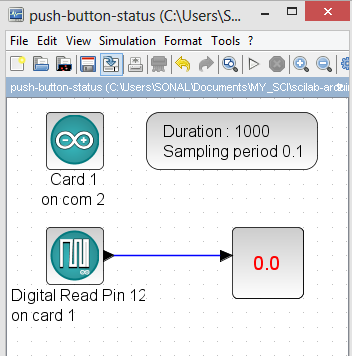
\includegraphics[width=\smfig]{\LocPushfig/push-button-status.PNG}
    \caption[Printing the push button status on the display block]
    {Printing the push button status on the display block.  This is
      what one sees when
        \LocPushscibrief{push-button-status.zcos}, is invoked.}
    \label{fig:push-button-status}
  \end{figure}

  We will next explain how to set the parameters for this simulation.
  To set value on any block, one needs to right click and open the
  {\tt Block Parameters} or double click.  The values for each block
  is tabulated in \tabref{tab:push-button-status}.  All other
  parameters are to be left unchanged.
  \begin{table}
    \centering
    \caption{Parameters to print the push button status on the display
      block} 
    \label{tab:push-button-status}
    \begin{tabular}{llc} \hline
      Name of the block & Parameter name & Value \\ \hline
      ARDUINO\_SETUP & Identifier of Arduino Card & 1 \\
      & Serial com port number & 2\portcmd \\ \hline
      TIME\_SAMPLE & Duration of acquisition(s) & 10 \\
      & Sampling period(s) & 0.1 \\ \hline
      DIGITAL\_READ\_SB & Digital pin & 12 \\
      & Arduino card number & 1 \\ \hline 
      AFFICH\_m & Block inherits (1) or not  (0) & 1 \\ \hline
    \end{tabular}
  \end{table}

\item In the second experiment, we take a step further and control the
  state of an LED in accordance with the status of the pushbutton. The
  Xcos implementation for this experiment is shown in
  \figref{fig:led-push-button}. Each time a user presses the
  pushbutton, the LED on digital pin 9 of the shield is switched
  on. If the shield is connected, the blue LED turns on.  When
  the pushbutton is released, the LED is switched off. Here, we note that
  the digital logic level of the pin of the \arduino\ board connected
  to pushbutton changes only for the time the pushbutton is being
  pressed.

  \begin{figure}
    \centering
    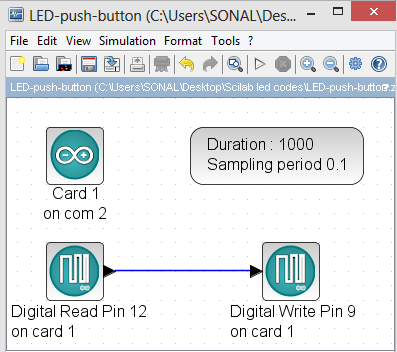
\includegraphics[width=\smfig]{\LocPushfig/led-push-button.PNG}
    \caption[Turning the LED on or off, depending on the pushbutton]
    {Turning the LED on or off, depending on the pushbutton.  This is
      what one sees when
        \LocPushscibrief{led-push-button.zcos}, is invoked.}
    \label{fig:led-push-button}
  \end{figure}

  We will next explain how to set the parameters for this simulation.
  To set value on any block, one needs to right click and open the
  {\tt Block Parameters} or double click.  The values for each block
  is tabulated in \tabref{tab:led-push-button}.  All other
  parameters are to be left unchanged.
  \begin{table}
    \centering
    \caption{Xcos parameters to turn the LED on through the pushbutton}
    \label{tab:led-push-button}
    \begin{tabular}{llc} \hline
      Name of the block & Parameter name & Value \\ \hline
      ARDUINO\_SETUP & Identifier of Arduino Card & 1 \\
      & Serial com port number & 2\portcmd \\ \hline
      TIME\_SAMPLE & Duration of acquisition(s) & 10 \\
      & Sampling period(s) & 0.1 \\ \hline
      DIGITAL\_READ\_SB & Digital pin & 12 \\
      & Arduino card number & 1 \\ \hline 
      DIGITAL\_WRITE\_SB & Digital pin & 9 \\
      & Card number & 1 \\ \hline
    \end{tabular}
  \end{table}
\end{enumerate}

\begin{exercise}
Let us carry out the following exercise:
\begin{enumerate}
\item In the above experiment, we controlled only one LED upon
  pushbutton press. Next, control multiple devices upon the pushbutton
  press. For example, upon press, turn on an LED and a motor and turn
  them off upon release.
\item Control several devices depending on the number of pushbutton
  press in a definite time span. For example, if the pushbutton is
  pressed once in time 't',say, turn on the LED. If it is pressed
  twice in time 't', turn on the motor. Here, you may want to consider
  the timing between two consecutive press.
\end{enumerate}
\end{exercise}

